\chapter{Implementace platformy}

\section{Konverzní mechanismus}

Jako zdroj pro implementaci konverzního mechanismu byl zvolen modul Munis ESML. Jedná se o část informačního systému pro města a obce společnosti Triada. spol. s.r.o.

\subsection{Munis ESML}

Účelem modulu Munis ESML je evidování odběratelských i dodavatelských smluv. Nabízí přehledné vyhledávání, statistiky, hlídání termínů, nebo možnost přiřadit smlouvy jednotlivým grantům, projektům či veřejným zakázkám (viz. Obr \ref{obr:munisEsml}).

\begin{figure}[H]
\centerline{\includegraphics[width=\textwidth]{img/munisEsml.eps}}
\caption{Modul ESML}
\label{obr:munisEsml}
\end{figure}

\newpage

\subsubsection{Struktura datového modelu}

Základem datového modelu jsou entity \textit{Smlouva} a \textit{Verze smlouvy}. Smlouva je základním stavovým objektem s hierarchickou strukturou. Vycházíme z předpokladu, že dodatek ke smlouvě je také smlouva, proto definujeme:

\begin{itemize}
\item Entita \textit{Smlouva} na kořenové úrovni popisuje smlouvu
\item Každý syn entity \textit{Smlouva} je jejím dodatkem
\end{itemize}

Každá smlouva je verzovaná, resp. entita Smlouva může mít několik \textit{Verzí smlouvy}. Entita \textit{Verze smlouvy} reprezentuje popisné údaje \textit{smlouvy}. Dále obsahuje vazby na \textit{rozdělovník, smluvní strany, milníky, transakce, externí kontakty a číselníky}, viz Obr. \ref{obr:munisDatamodel}.

Každá Verze smlouvy může obsahovat hierarchickou strukturu příloh. Každá entita Příloha smlouvy reprezentuje fyzický soubor. Přílohy definujeme takto:

\begin{itemize}
\item Každá \textit{Verze smlouvy} může mít pouze jednu kořenovou přílohu
\item Kořenová příloha je hlavním dokumentem obsahujícím text smlouvy
\item Ostatní jsou dílčími přílohami
\end{itemize}

Entity \textit{Změna stavu smlouvy, Rozdělovník, Rozdělovník smluv přístup, Rozdělovník smluv přístup historie} nejsou pro naše účely důležité, proto je dále v textu nebudeme zmiňovat.

\subsubsection{Omezení vůči standardu}

V porovnání s datovým standardem pro smlouvy disponuje Munis ESML několika omezeními:

\begin{itemize}
\item Modul nepodporuje objednávky a faktury
\item Transakce nejsou implementovány - s podporou transakcí a obecně smluvního plnění se počítá do dalších verzí 
\end{itemize}

\begin{figure}[H]
\centerline{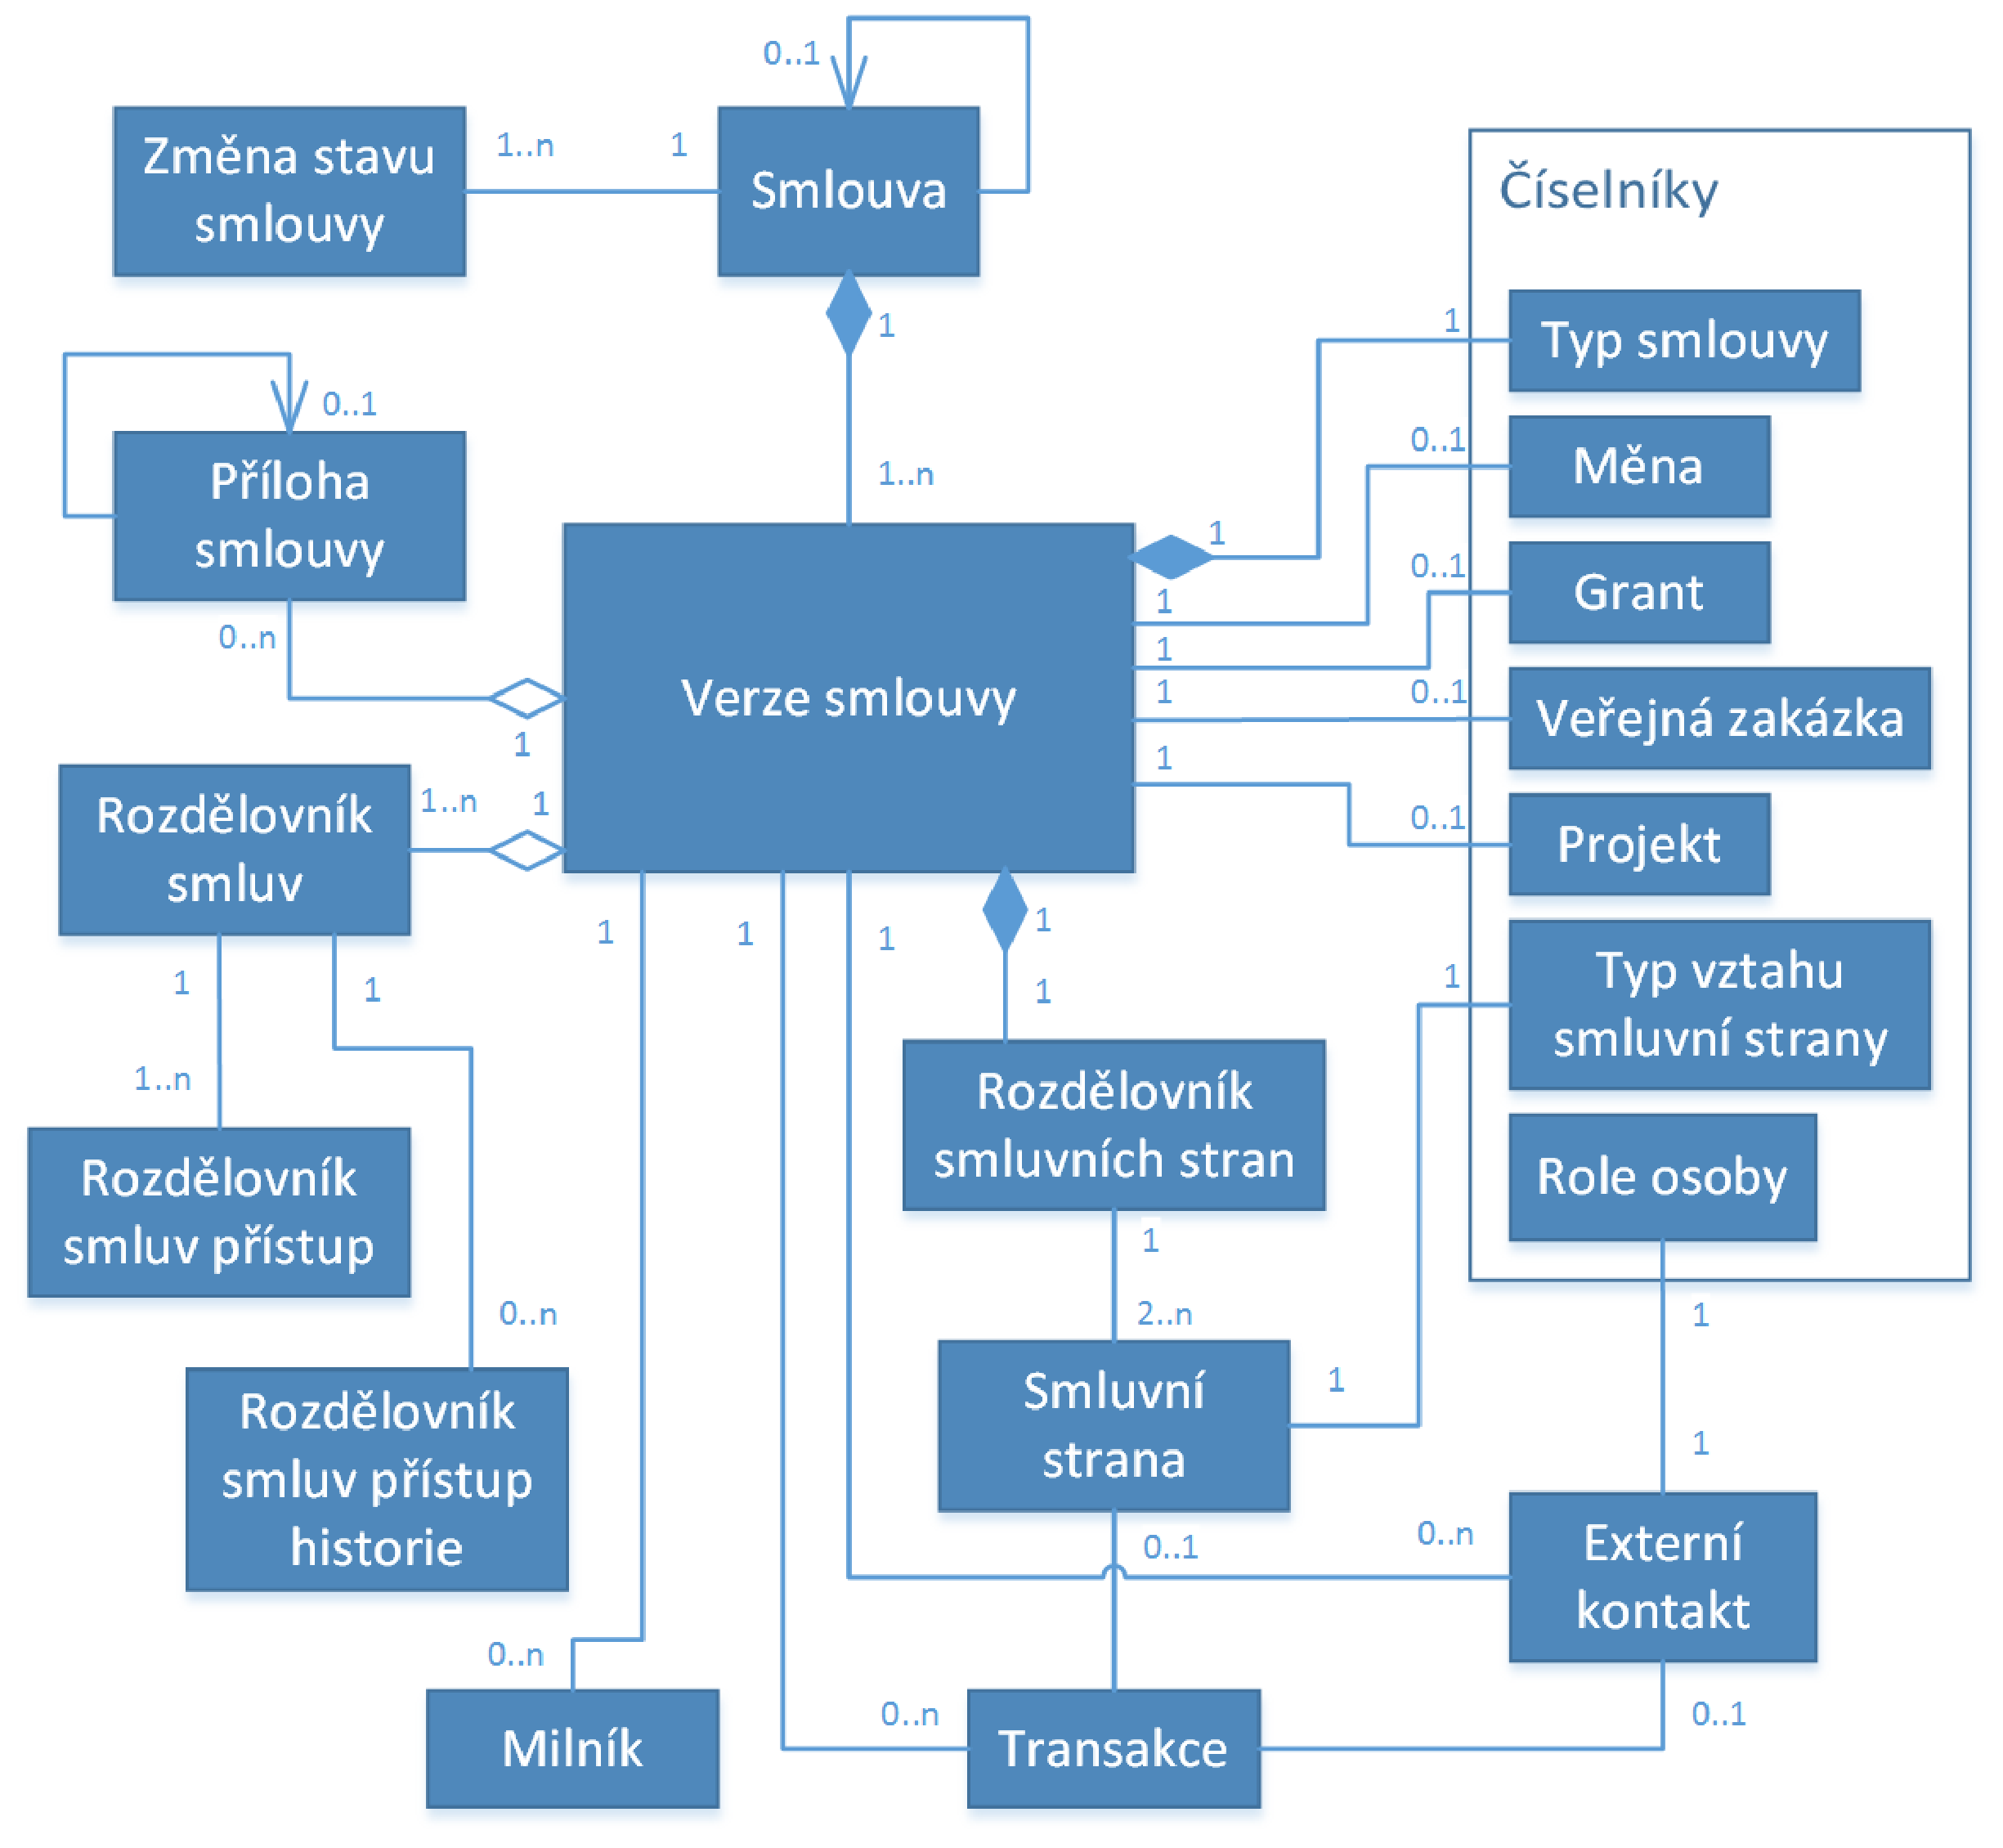
\includegraphics[width=\textwidth]{img/munisDatamodel.eps}}
\caption{ Zjednodušený datový model (bez atributů) Munis ESML}
\label{obr:munisDatamodel}
\end{figure}

\subsection{R2RML mapování}

Pomocí R2RML skriptu můžeme namapovat konkrétní sloupce z databázových tabulek na RDF predikáty. Pro složitější mapování umožňuje R2RML definovat vlastní SQL pohledy (SQL Views) nad relační databází, čehož využijeme. Pro každou entitu v rámci datového standardu proto definujeme vlastní SQL pohled. Výsledný R2RML skript lze nalézt v příloze E.

V následující části je schématicky naznačeno mapování položek. Každé entitě přiřadíme URI a typ. Následně se namapují jednotlivé položky na predikáty. Vycházíme z informací řečených v kapitole~\nameref{sec:kap4}. TODO - otázka kolekcí

\subsubsection*{Smlouva}

\begin{itemize}
\item URI entity - url{http://[domain]/contract/{ID}/{PORADIVERZE}}
\item Typ - cn:Contract
\end{itemize}

Konstanty:
\begin{itemize}
\item Type (dcmi:type) - s hodnotou “Smlouva”
\item PriceAnnual (cn:priceAnnual) - Nelze určit roční částku, proto vždy “false”
\end{itemize}

Nenamapované položky:
\begin{itemize}
\item AmountNoVat (gr:hasCurrencyValue) - cena bez dph, předpokládaná podpora spolu s podporou podrobného smluvního plnění
\item SubjectType (cn:subjectType) - Číselník typů zboží/služeb, předpokládaná podpora u dalších verzí
\item PlainText (cn:plainText) - Prostý text dokumentu smlouvy, resp. alternativa k oskenovaným dokumentům. Vyžaduje hlubší analýzu procesu zpracování dokumentů 
\item Funding (cn:funding) - Vychází zatím z nedefinovaného číselníku datového standardu
\end{itemize}

Poznámky:
\begin{itemize}
\item URI (cn:uri) - položka je stejná jako u URI entity
\item Valid (cn:valid) - položka je “true”, jestliže se jedná o nejnovější verzi smlouvy, jinak je “false”
\item Competency (cn:competency) - vyplní se na základě položky Typ u databázové tabulky Typ smlouvy. Pokud je Typ smlouvy - “Veřejnoprávní smlouva” vyplní se i k položkce Competency, jinak se vyplní “Soukromoprávní smlouva”
\end{itemize}

Mapování kolekcí a odkazů:
\begin{itemize}
\item Document (com:contentUrl) - URI odkazu -\\\textit{http://[domain]/file/{SADADUL\_ULOZISTEID}/{NAZEVSOUBORU}}
\item Versions (cn:version) - URI odkazu -\\\textit{http://[domain]/contract/{ID}/{PORADIVERZE}/version}
\item Publisher (dc:publisher) - URI odkazu -\\\textit{http://[domain]/publisher}
\item Parties (cn:Party) - URI odkazu -\\\textit{http://[domain]/party/{HAD\_POUZITA}}
\item Amendments (cn:amendment) - URI odkazu -\\\textit{http://[domain]/amendment/{ID}/{PoradiVerzeDodatku}}
\item Attachments (cn:attachment) - URI odkazu -\\\textit{http://[domain]/attachment/{ID}/1}
\item ResponsiblePersons (cn:responsiblePerson) - Každá veřejná zakázka má vazbu na externí kontakty. Externím kontaktem může být buď uživatel informačního systému (tabulka TRI\_UZIVATEL), nebo jakákoli osoba vyplněná v tabulce Externí kontakt. Pro potřeby mapování se hodnoty spojí do jednoho stringu, viz Obr. 7.3.
\item Implementation (cn:implementation) - Uri odkazu -\\\textit{http://[domain]/contract/{ID}/{PORADIVERZE}/implementation}
\end{itemize}

\begin{figure}[H]
\centerline{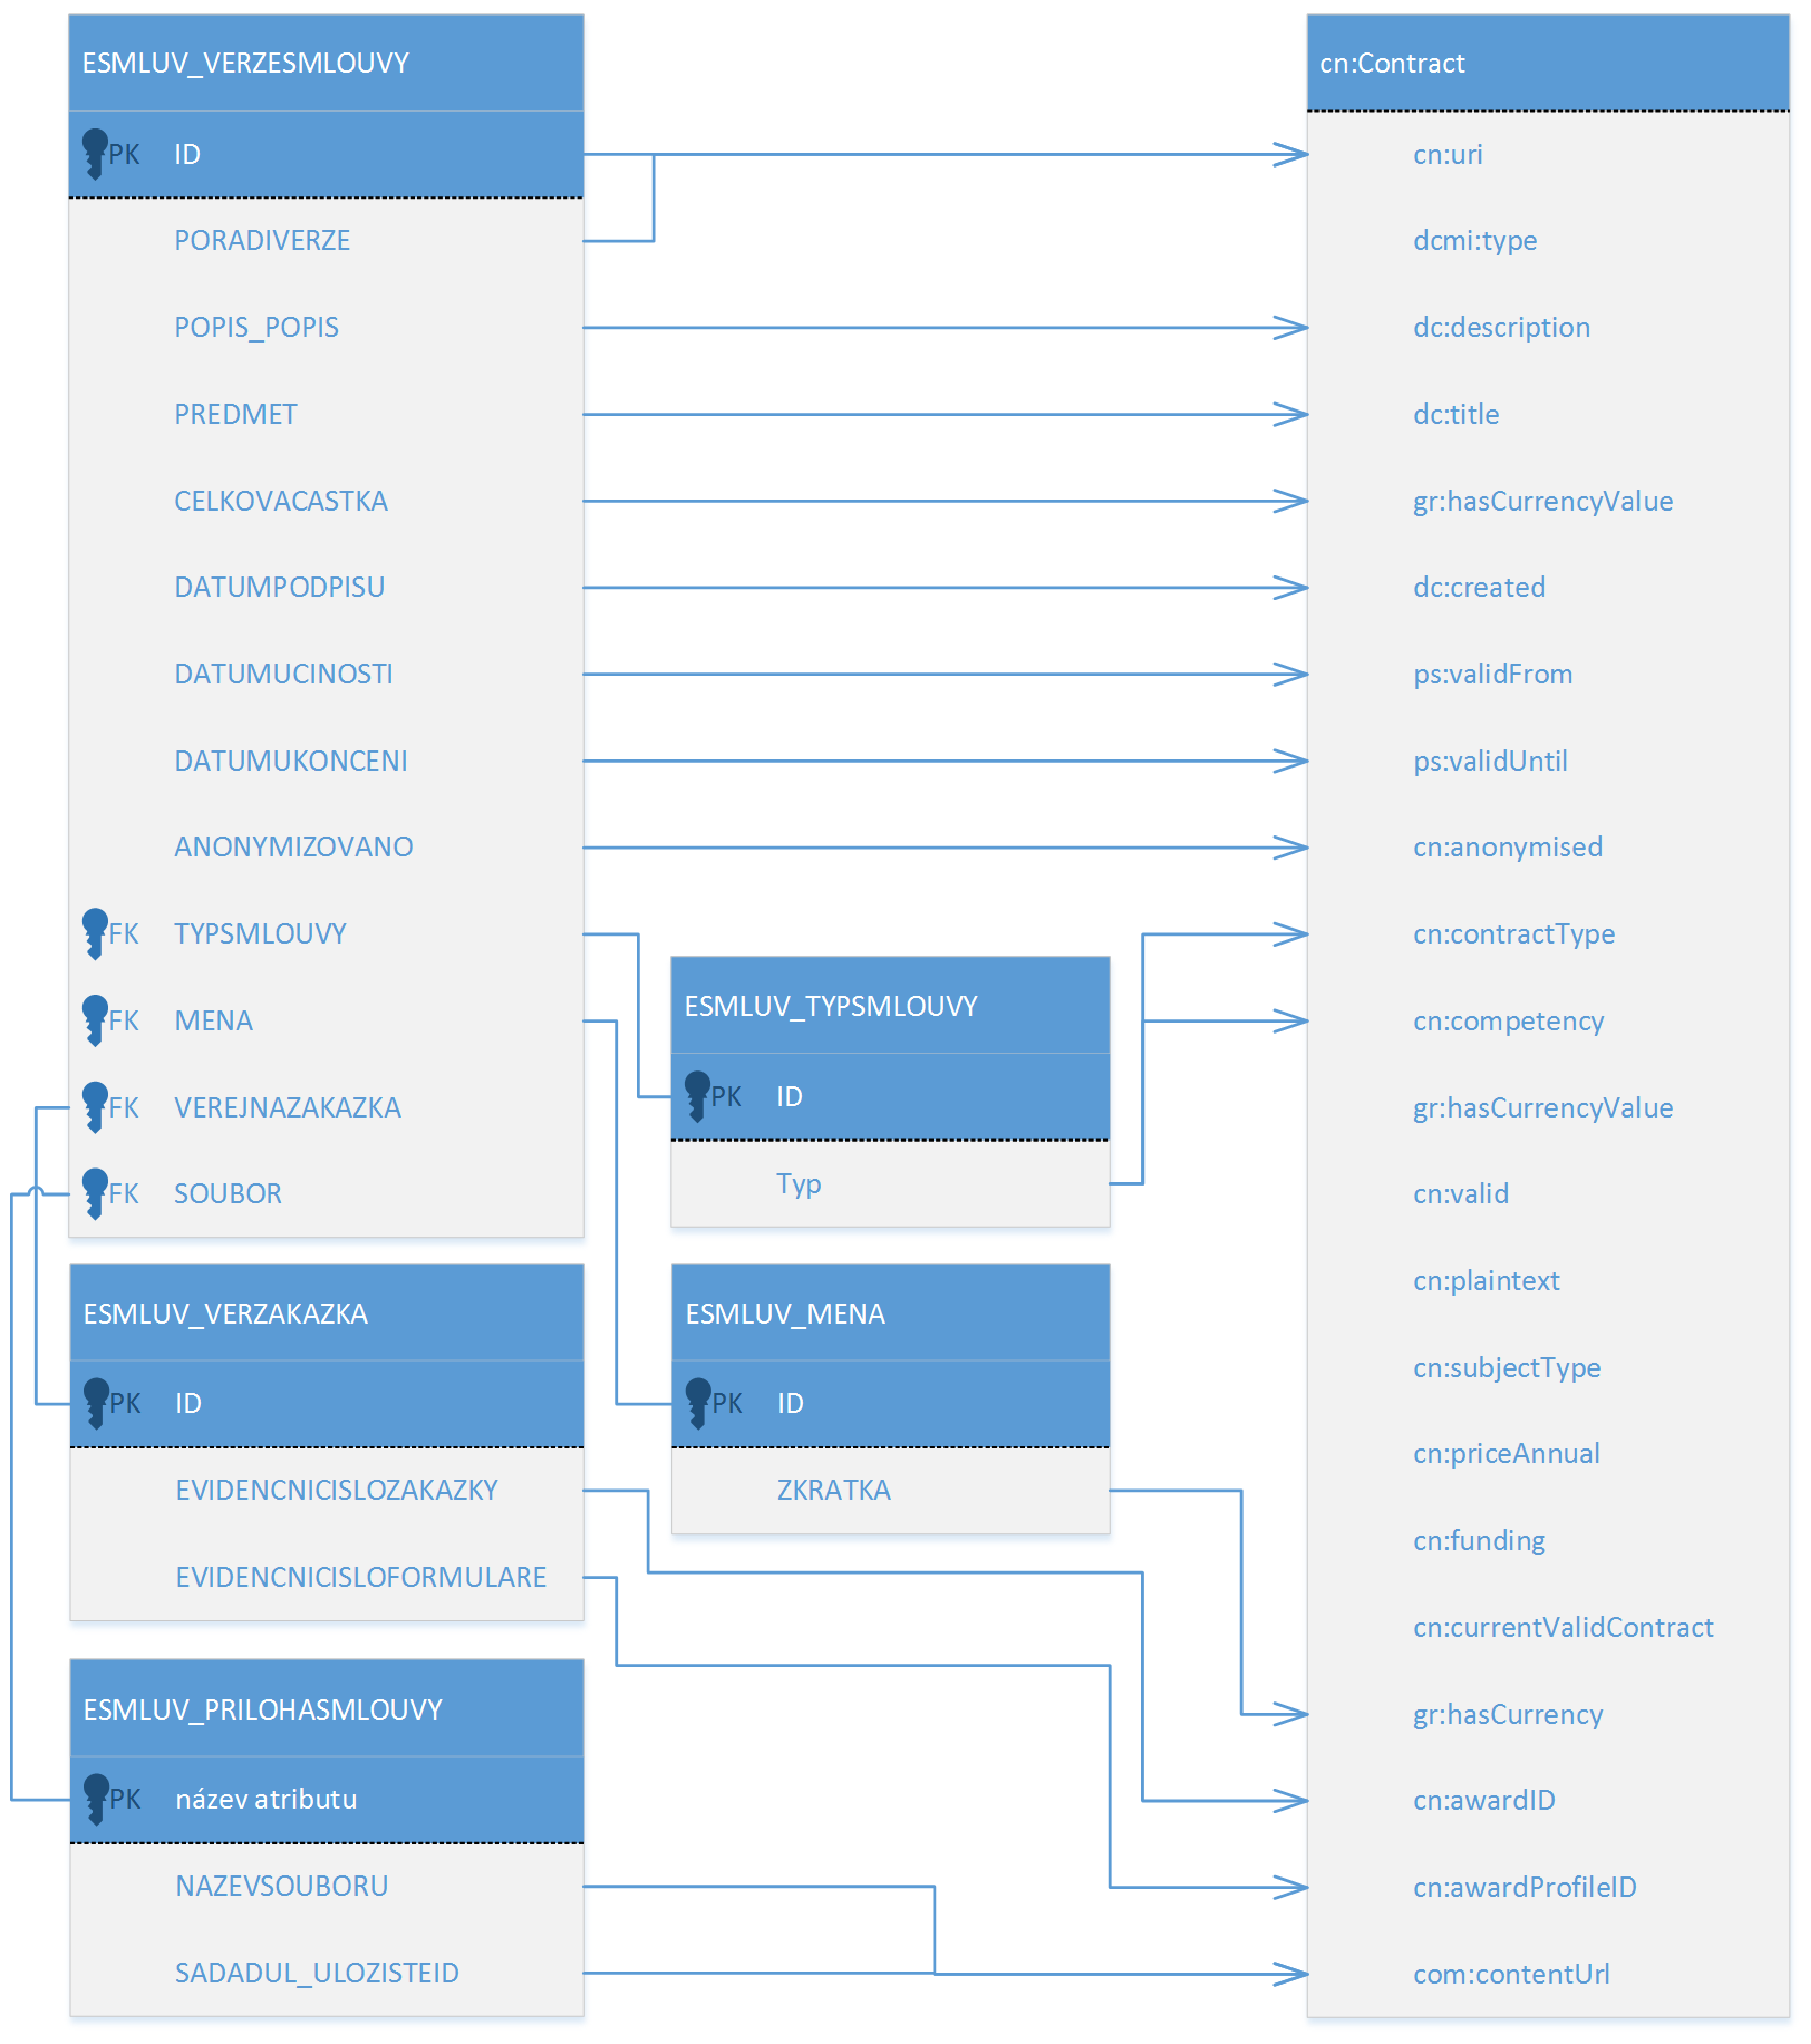
\includegraphics[width=\textwidth]{img/mapContract.eps}}
\caption{R2RML mapování vlastností Smlouvy}
\label{obr:mapContract}
\end{figure}

\begin{figure}[H]
\centerline{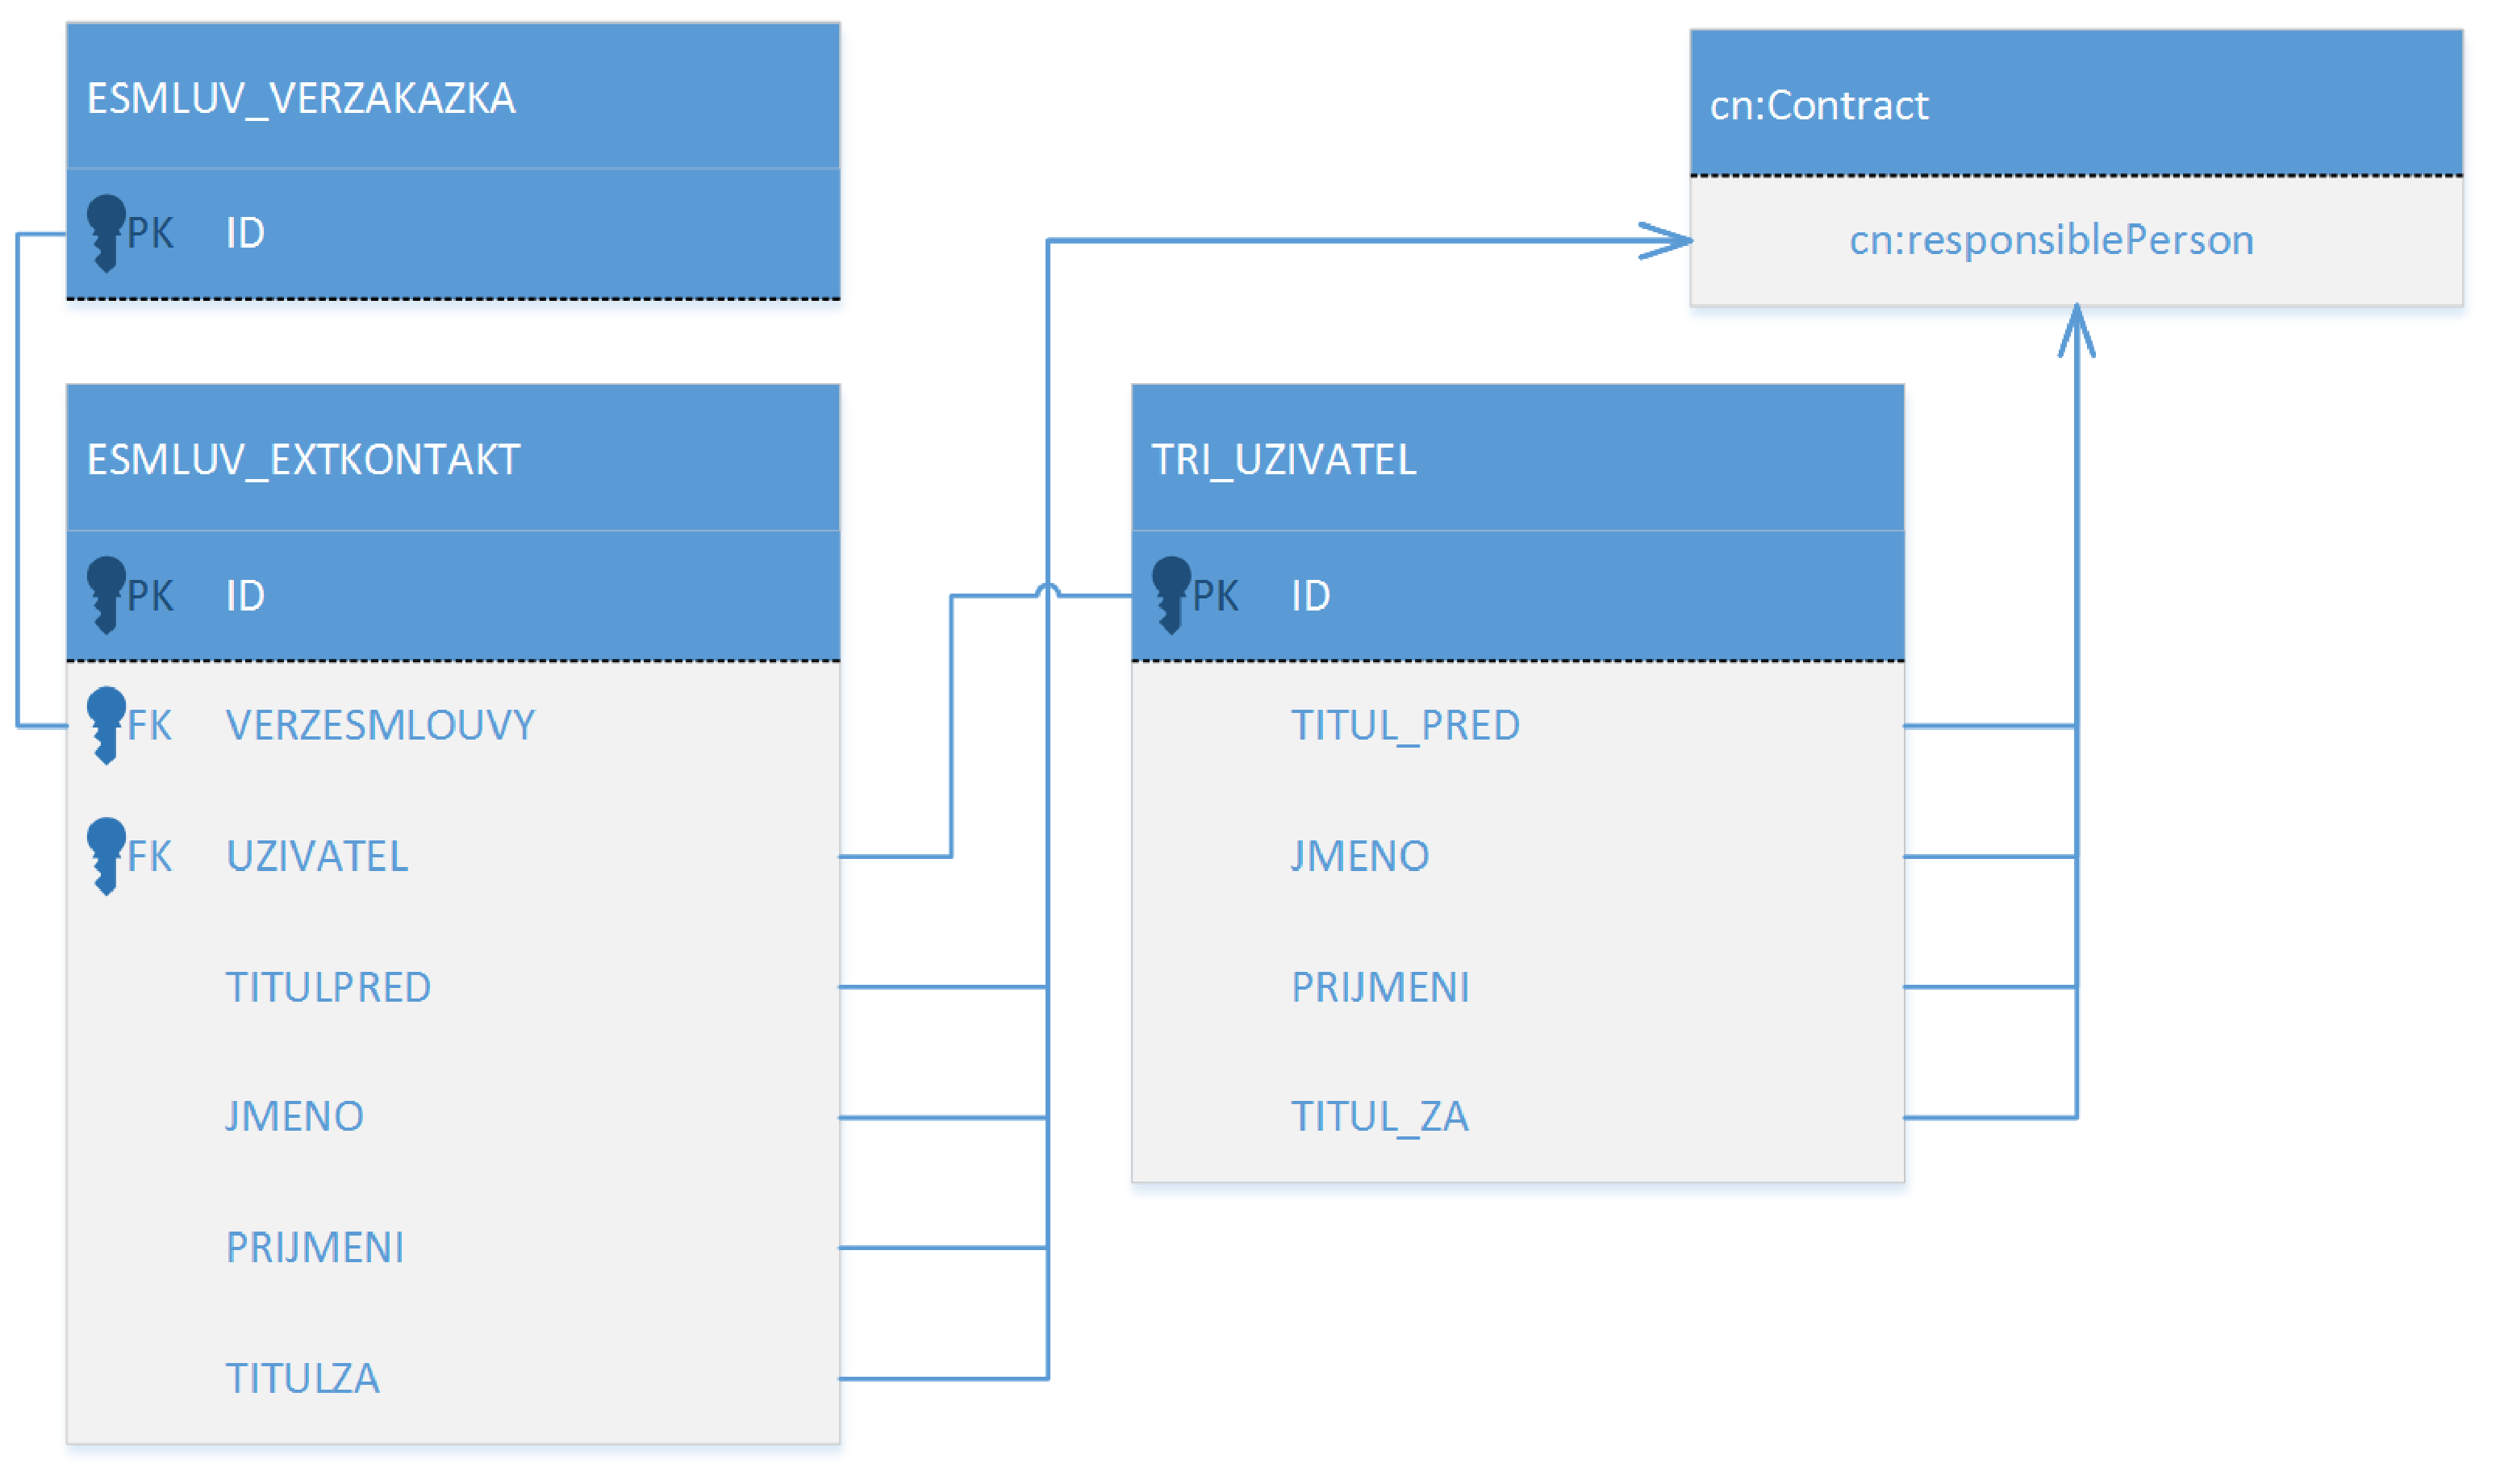
\includegraphics[width=\textwidth]{img/mapRespPerson.eps}}
\caption{R2RML mapování vlastností Smlouvy (Externího kontaktu)}
\label{obr:mapRespPerson}
\end{figure}

\subsubsection*{Verze}

\begin{itemize}
\item URI entity -\\\textit{http://[domain]/[type]/{ID}/{PORADIVERZE}/version}
\item Typ - cn:Version
\end{itemize}

Nenamapované položky:
\begin{itemize}
\item PublisherId (cn:publisherId) - Díky id a verzi smlouvy máme každou entitu jednoznačně identifikovanou, proto není třeba vyplňovat
\end{itemize}

Poznámky:
\begin{itemize}
\item URI (cn:uri) - položka je stejná jako u URI entity
\end{itemize}

\begin{figure}[H]
\centerline{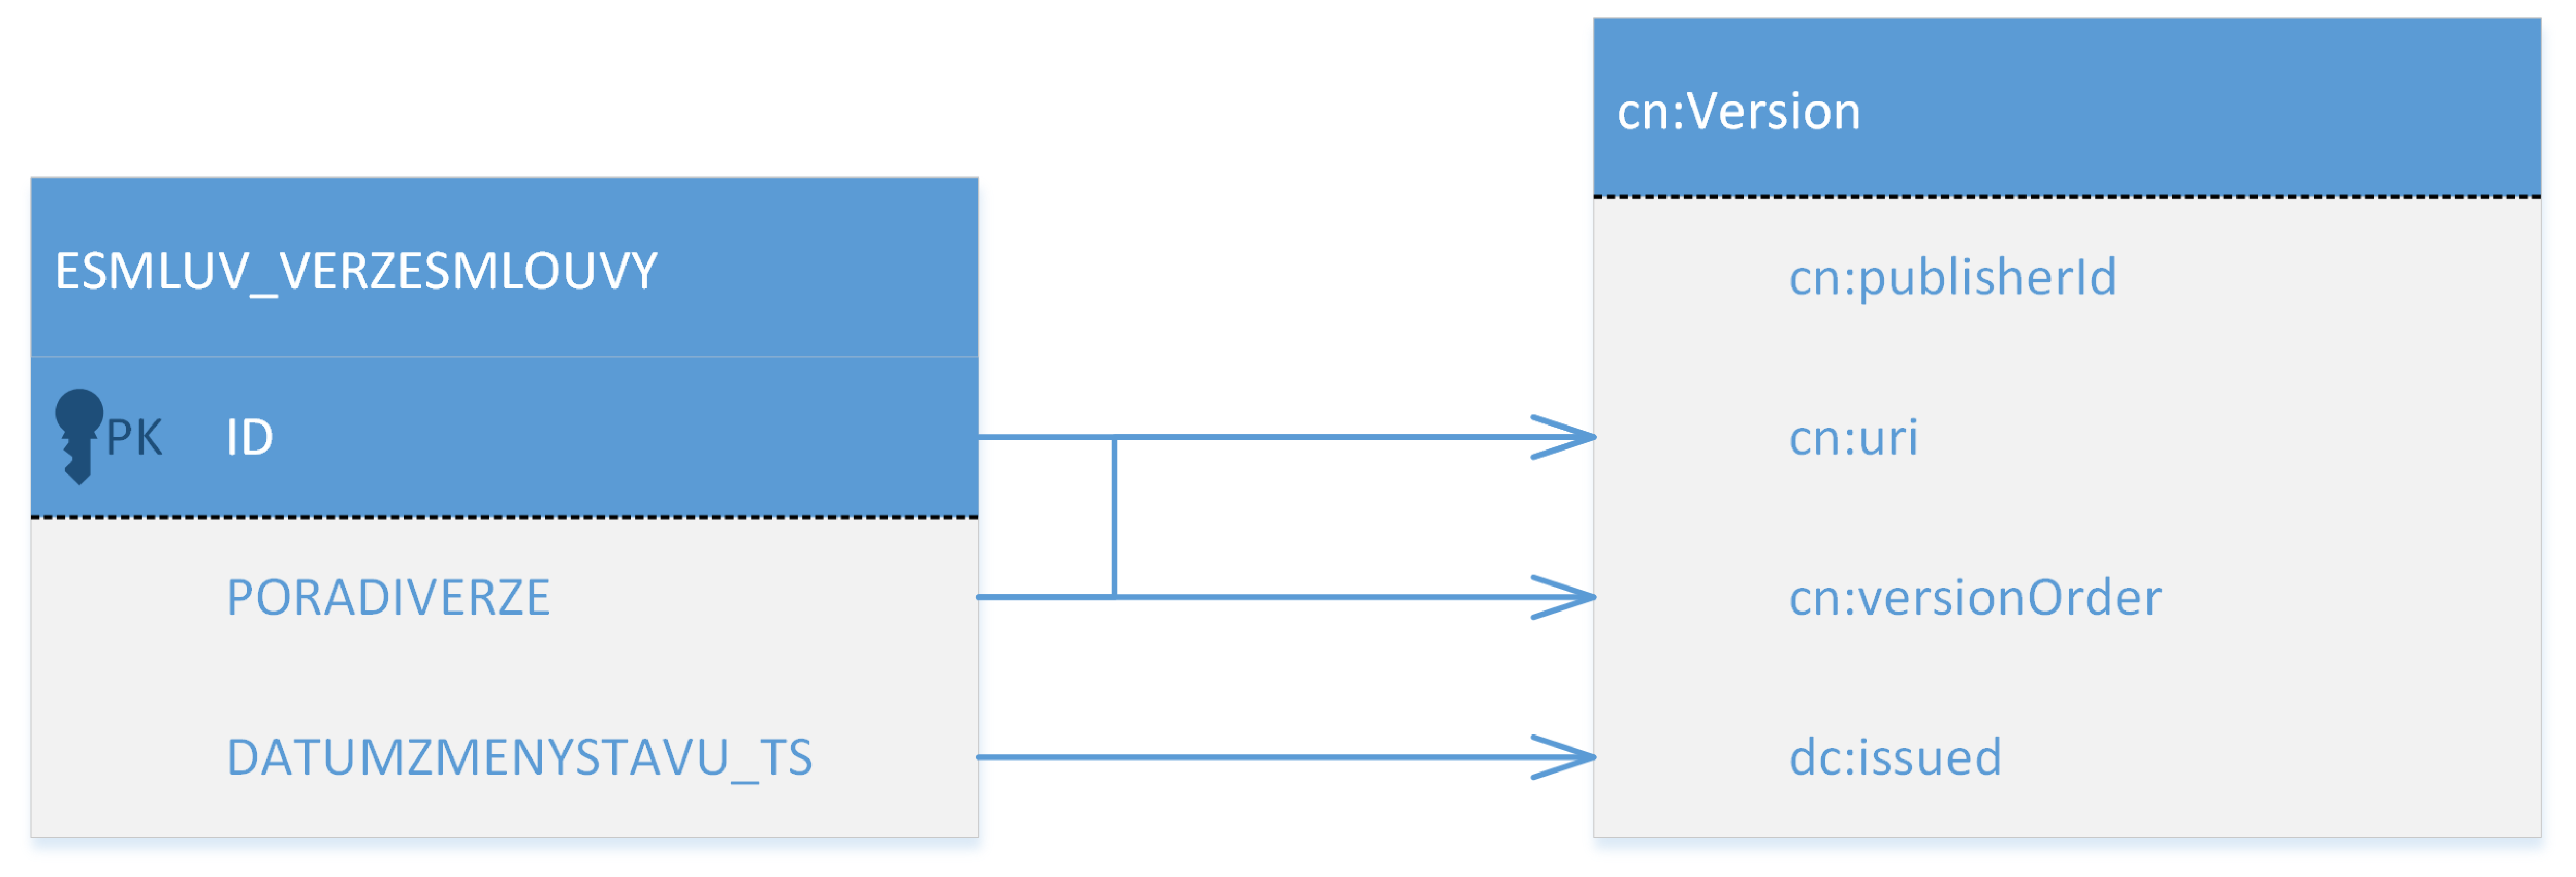
\includegraphics[width=\textwidth]{img/mapVersion.eps}}
\caption{R2RML mapování vlastností Verze}
\label{obr:mapVersion}
\end{figure}

\subsubsection*{Smluvní strana}

\begin{itemize}
\item URI - \textit{http://[domain]/party/{HAD\_POUZITA}}
\item Typ strany- gr:BusinessEntity

\end{itemize}

Nenamapované položky:
\begin{itemize}
\item Payer (cn:payer) - Modul ESML zatím neeviduje smluvní plnění, takže nelze určit 
\item SuperInstitution (cn:superiorInstitution) - Modul ESML neeviduje nadřazené instituce
\end{itemize}

\subsubsection*{Adresa}

\begin{itemize}
\item URI - \textit{http://[domain]/party/{HAD\_POUZITA}/address}
\item Typ - schema:PostalAddress

\end{itemize}

Nenamapované položky:
\begin{itemize}
\item Nuts (cn:nuts) - Modul ESML neeviduje hodnoty normalizované klasifikace územních celků
\end{itemize}

\begin{figure}[H]
\centerline{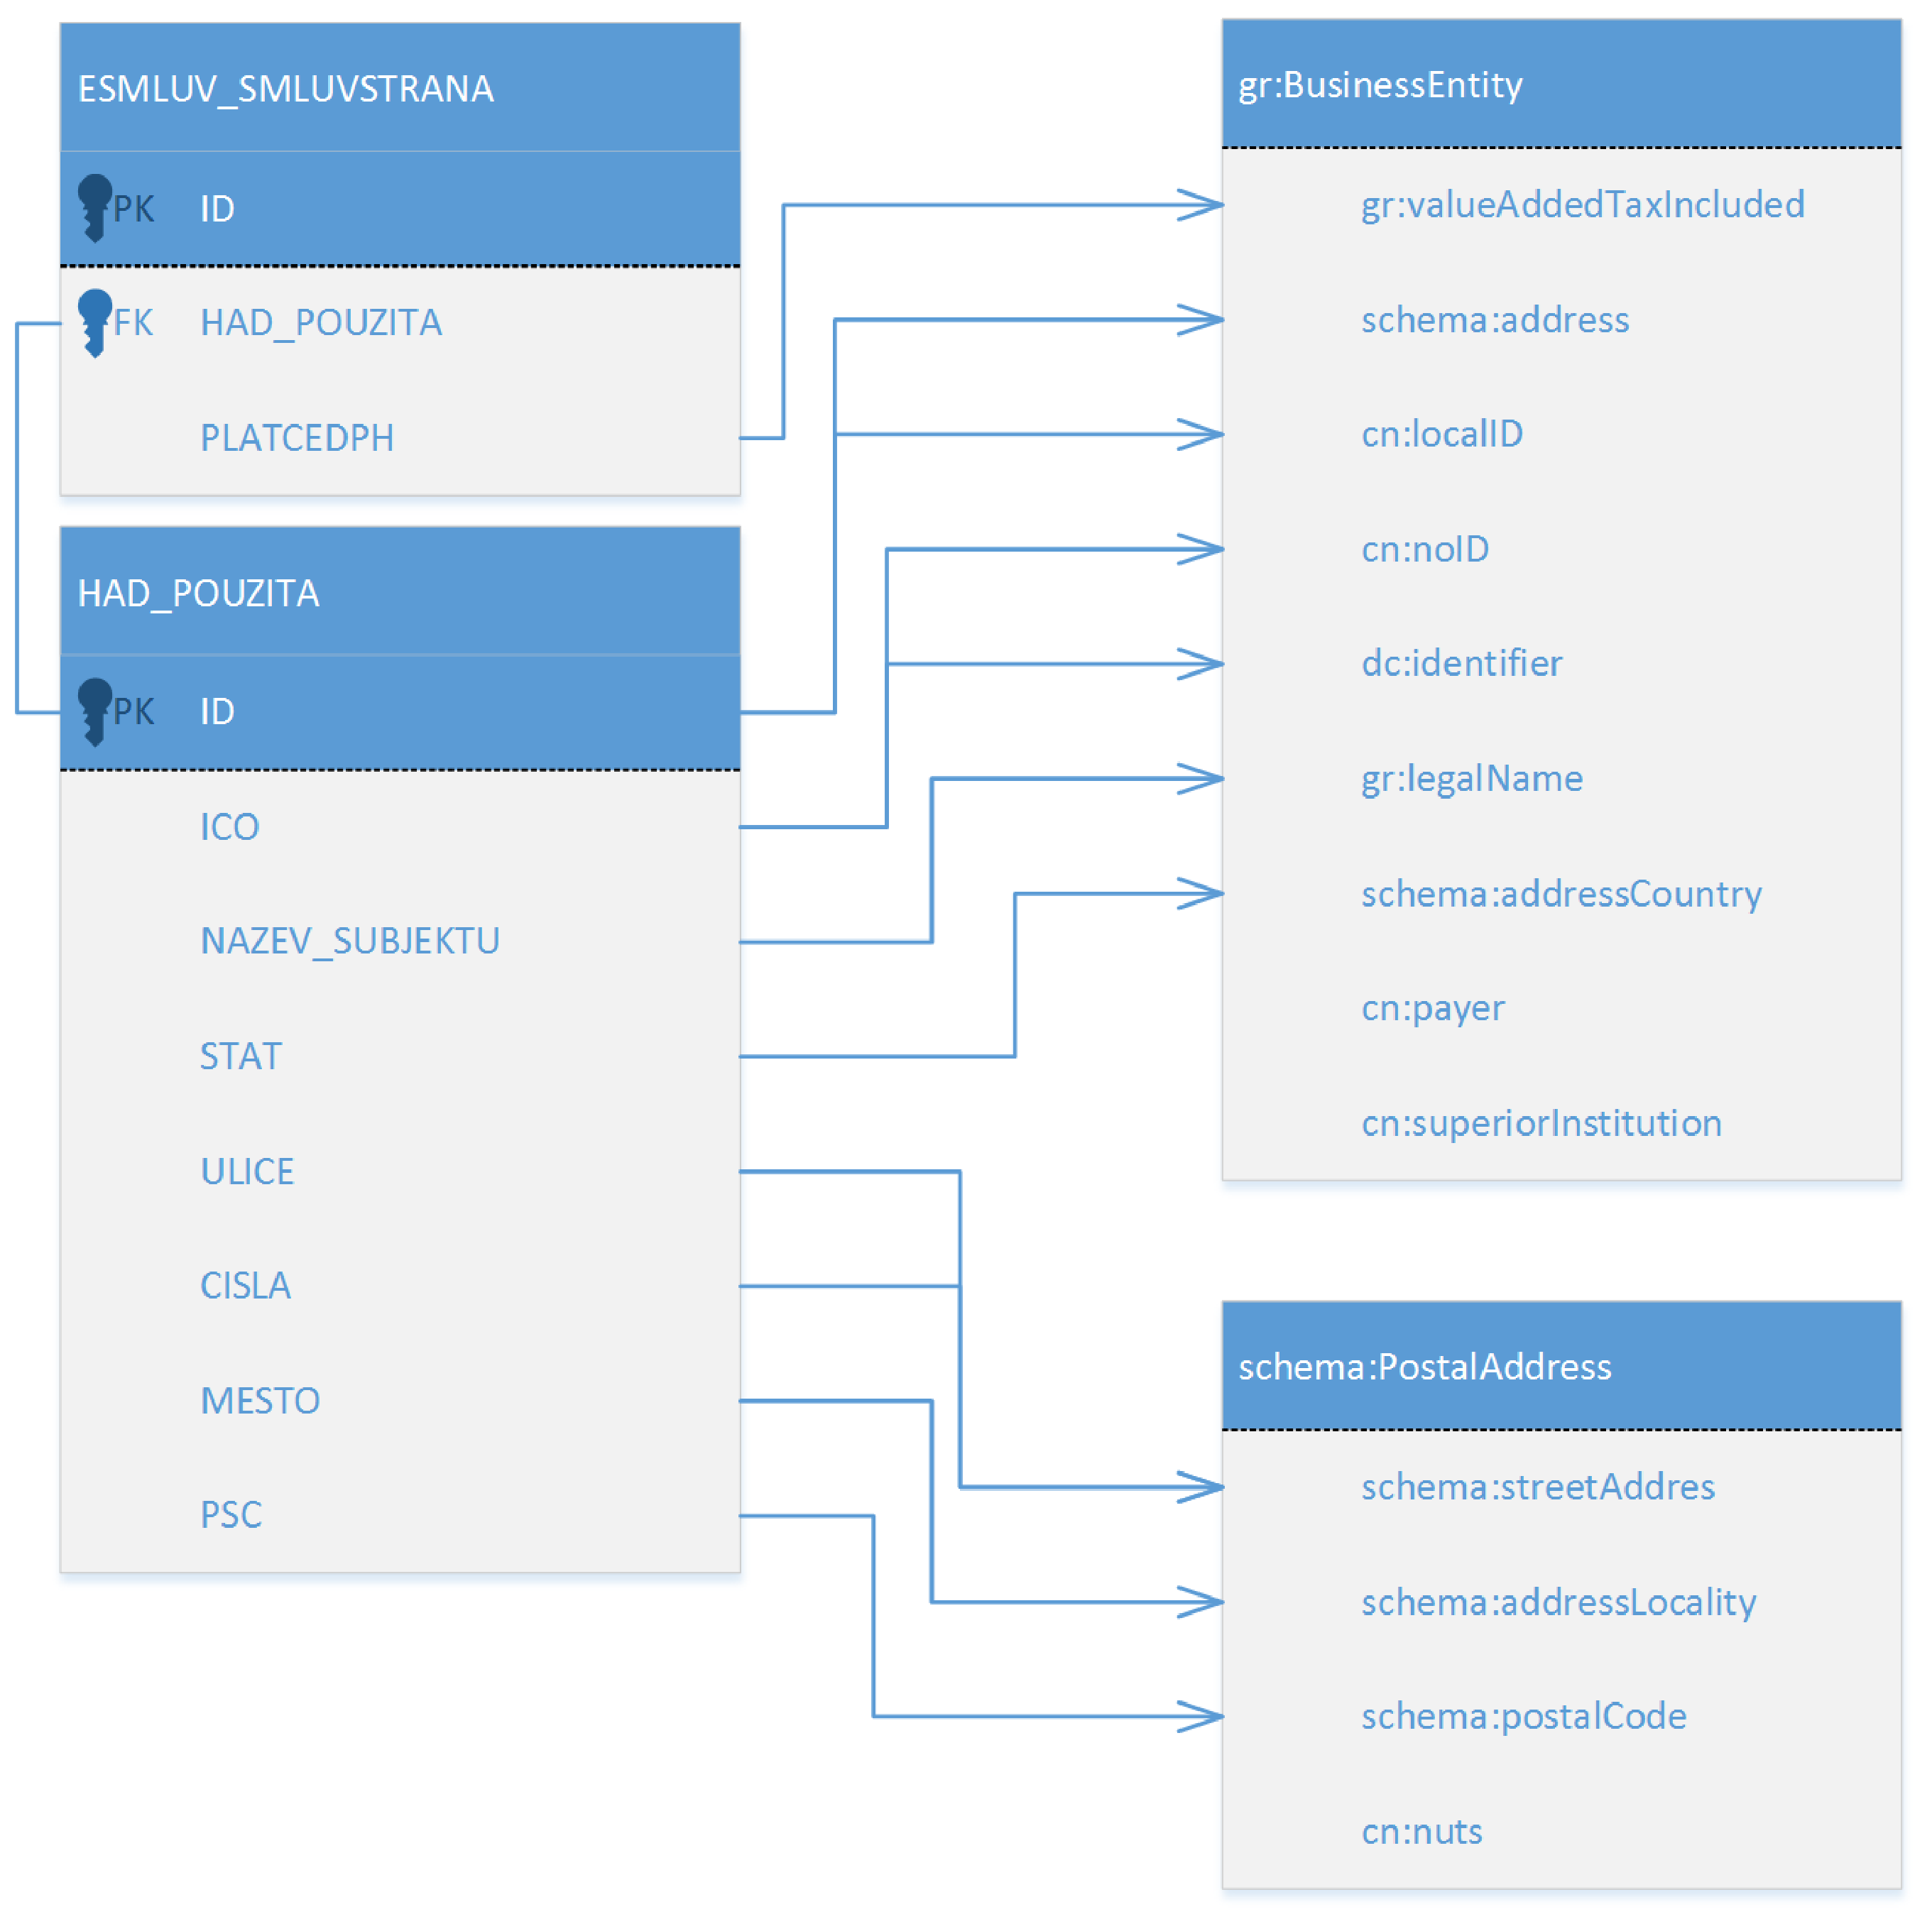
\includegraphics[width=\textwidth]{img/mapParty.eps}}
\caption{R2RML mapování vlastností Smluvní strany a Adresy}
\label{obr:mapParty}
\end{figure}

\subsubsection*{Příloha}

\begin{itemize}
\item URI entity  - \textit{http://[domain]/attachment/{ID}/1}
\item Typ - cn:Attachment
\end{itemize}

Konstanty
\begin{itemize}
\item Type (dcmi:type) - s hodnotou “Příloha”
\item Valid (cn:valid) - položka je “true”, přílohy nejsou verzované
\end{itemize}

Nenamapované položky:
\begin{itemize}
\item PlainText (cn:plainText) - Prostý text dokumentu přílohy, resp. alternativa k oskenovaným dokumentům. Vyžaduje hlubší analýzu procesu zpracování dokumentů 
\end{itemize}

Poznámka:
\begin{itemize}
\item URI (cn:uri) - položka je stejná jako u URI entity
\end{itemize}

Mapování kolekcí a odkazů:

\begin{itemize}
\item Document (com:contentUrl) - URI odkazu -\\\textit{http://[domain]/file/{SADADUL\_ULOZISTEID}/{NAZEVSOUBORU}}
\item Versions (cn:version) - URI odkazu -\\\textit{http://[domain]/attachment/{ID}/1/version}
\item Publisher (dc:publisher) - URI odkazu -\\\textit{http://[domain]/attachment/{ID}/1/publisher}
\item Contract (cn:contract) - URI nadřízené smlouvy -\\\textit{http://[domain]/contract/{SmlouvaID}/{PORADIVERZE}}
\end{itemize}

\begin{figure}[H]
\centerline{
\includegraphics[width=\textwidth]{img/mapAttachment.eps}}
\caption{R2RML mapování vlastností Příloha}
\label{obr:mapAttachment}
\end{figure}

\subsubsection*{Dodatek}

\begin{itemize}
\item URI entity  -\\\textit{http://[domain]/amendment/{ID}/{PoradiVerzeDodatku}}
\item Typ - cn:Amendment
\end{itemize}

Poznámka:
V rámci relační databáze je Dodatek stejná entita jako smlouva. Tudíž použijeme obdobné mapování jako u smlouvy.

\subsubsection*{Implementace}

\begin{itemize}
\item URI entity - \textit{http://[domain]/contract/{ID}/{PORADIVERZE}/implementation}
\item Typ - cn:Implementation
\end{itemize}

\subsubsection*{Milník}

\begin{itemize}
\item URI entity  - \textit{http://[domain]/contract/{ID}/{PORADIVERZE}/implementation/milestone/{MilestoneID}}
\item Typ - cn:Milestone
\end{itemize}

\begin{figure}[H]
\centerline{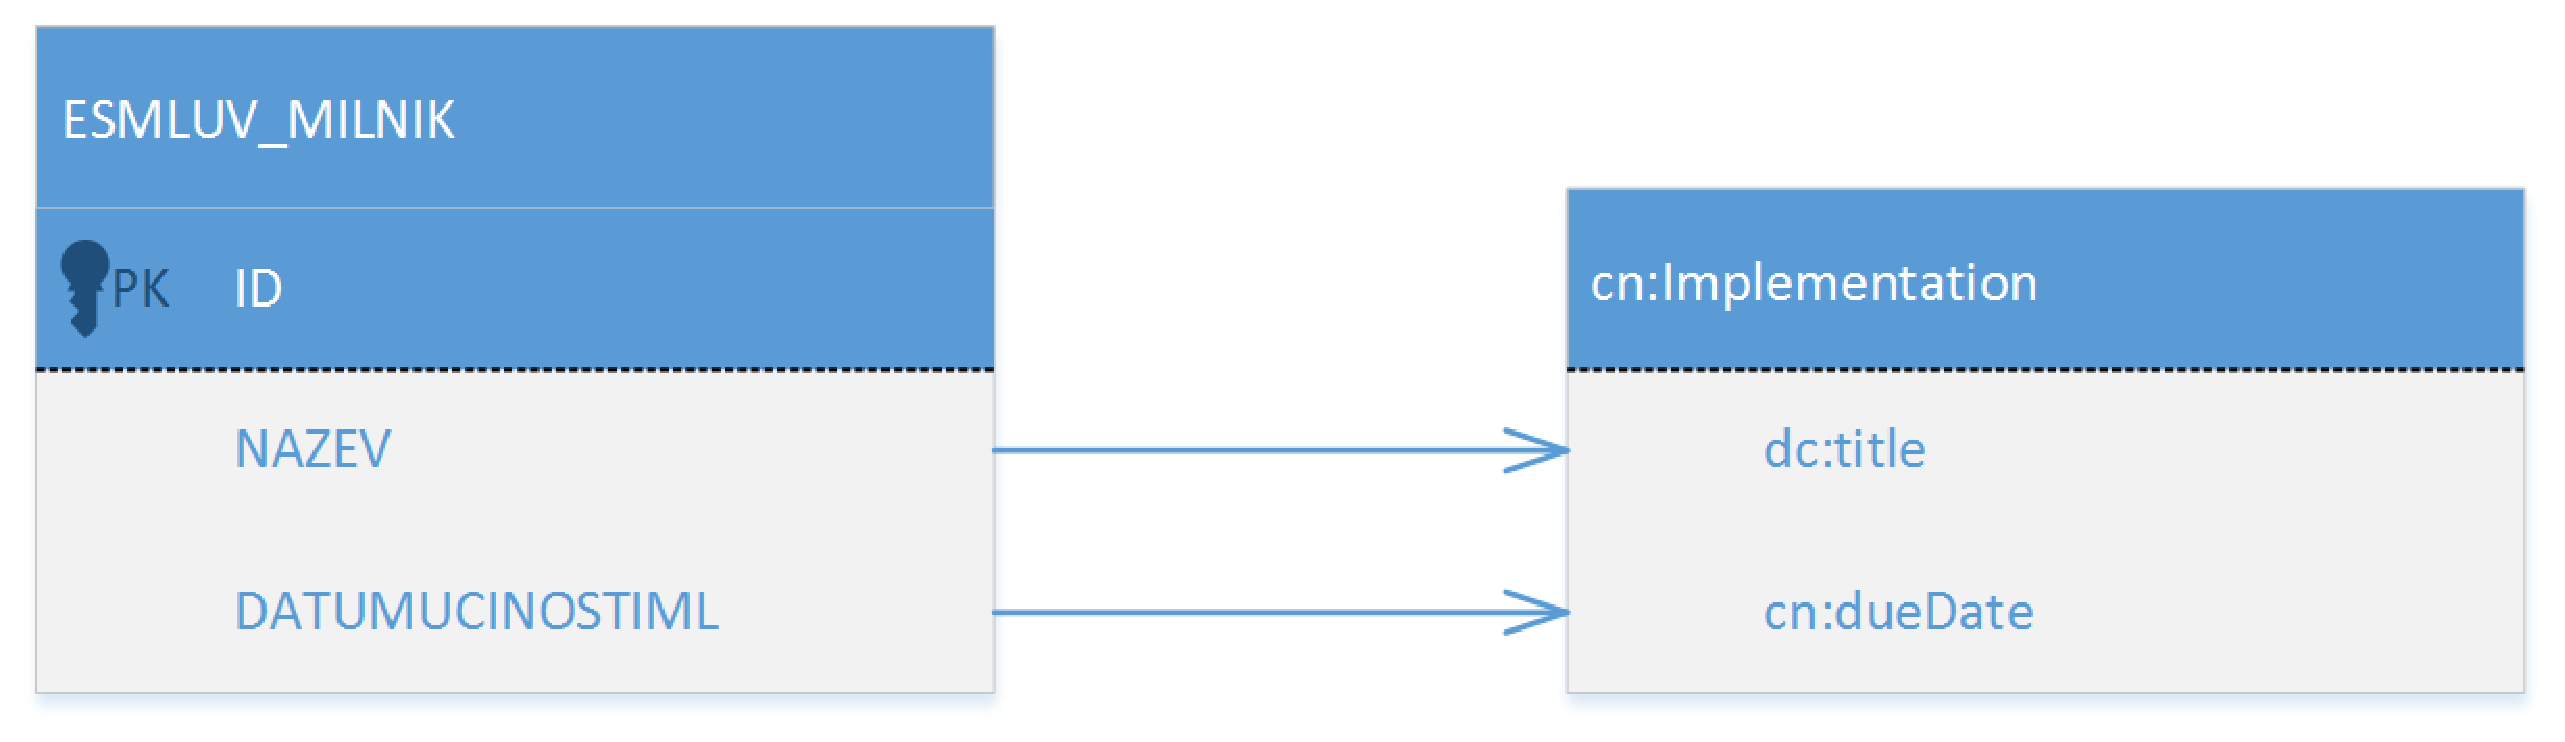
\includegraphics[width=\textwidth]{img/mapMilestone.eps}}
\caption{R2RML mapování vlastností Milníku}
\label{obr:mapMilestone}
\end{figure}

\subsubsection*{Vydavatel}

\begin{itemize}
\item URI entity  - \textit{http://[domain]/publisher}
\item Typ - foaf:Organization
\end{itemize}

Konstanty:
\begin{itemize}
\item Country (schema:addressCountry) - Hodnota “CZE”
\end{itemize}

Nenamapované položky:
\begin{itemize}
\item Authentication (cn:authentication) - Pro naše účely nemá smysl
\end{itemize}

Poznámky:
\begin{itemize}
\item TODO sameAs
\end{itemize}

\subsection{Volba R2RML procesoru}

K R2RML mapování využijeme projektu DotNetR2RMLStore\footnote{https://github.com/mchaloupka/DotNetR2RMLStore}. Jedná se o experimentální R2RML procesor pracující nad relačními databázemi Microsoft SQL\footnote{Většina veřejných institucí využívající produkty firmy Triada. spol, s.r.o. pracuje nad databázemi MS SQL. Proto nebereme MS SQL jako omezení. Munis ESML ale umožňuje práci i nad databází Oracle.}. Tento projekt je vytvářený v rámci Katedry softwarového inženýrství na Matematicko-fyzikální fakultě. 

\subsubsection{Omezení R2RML procesoru}

Využití zmíněného R2RML procesoru si vyžádalo několik drobných omezení. 

Pro náš případ využijeme DotNetR2RMLStore ve verzi 0.0.0.9. Zkoušená vyšší verze mění logiku zpracování dotazů a zatím nepodporuje SQL Views\footnote{TODO}. Je tu i možnost vytvořit SQL views přímo nad databází subjektu a mapovat R2RML skriptem přímo tyto pohledy. Není to problém, ale nelze považovat za samozřejmost, že subjekt zpřístupní databází k úpravám. 

Procesor nepodporuje SPARQL příkazy ASK a DESCRIBE. Pro naše účely ale stačí hlavní příkazy SELECT a CONSTRUCT.

Samotný R2RML skript musí mít v hodnotě template vždy vyplněné absolutní URI. Prefixovaný zápis procesor zpracuje, ale při zpracovaní dotazů daný template nerozpozná.

Formáty datumových položek v RDF datech by měly splňovat W3C specifikaci, což aktuálně nesplňují. Vrácené datumové hodnoty tedy v rámci postprocesingu nahradíme správným formátem\footnote{http://www.w3.org/TR/NOTE-datetime}. 

\subsection{Volba technologií a implementační platformy}

Vzhledem k tomu, že projekt DotNetR2RMLStore je implementován v prostředí .Net, tak zvolíme tuto platformu i pro implementaci konverzního mechanismu. Konverzní mechanismus bude mít formu webové aplikace, resp. virtuálního SPARQL endpointu, kterou budeme implementovat v technologii ASP.Net. Využijeme tradičního architektonického vzoru MVC. K práci s RDF daty budeme využívat knihovnu dotnetRdf.

\subsection{Napojení na datové úložiště}

Mezi specifika informačních systémů firmy Triada s.r.o můžeme zmínit, že neukládají fyzické soubory (v našem případě smlouvy) do databáze s ostatními daty, ale do specializovaného datového úložiště. Nutnou podmínkou pro zobrazení těchto dat je proto propojení konverzního modulu s databází datového úložiště. Využijeme k tomu knihovnu TriadaModulZaklad.

V relační databázi jsou uloženy informace o daném souboru. Jedná se mimo jiné o název souboru a jeho jednoznačný indentifikátor v datovém úložišti ve formě GUID. Informace tedy namapujeme již na zmíněné URI -\\\textit{http://[domain]/file/{SADADUL\_ULOZISTEID}/{NAZEVSOUBORU}}. Při přístupu na danou adresu se informace převedou na dotaz do datového úložiště a uživateli se vrátí konkrétní soubor ke stažení.

\subsection{SPARQL endpoint}

\subsection{Zpracování RDF výstupu}

Příkazy SELECT jsou zpracovávány proudově v tabulkové formě, resp. seznamem definovaných proměnných a výčet hodnot, které jim odpovídají. Definujeme proto handler naslouchající nad R2RML procesorem, kterým výsledky dotazu postupně zpracováváme. Pro každý výstupní formát proto implementujeme handler serializující výsledky do zvoleného datového formátu. Aplikace podporuje základní formáty jako HTML, Turtle, N-Triples, RDF/XML, XML, JSON a CSV. Formáty XML, JSON, CSV serializujeme podle doporučení W3C\footnote{http://www.w3.org/TR/sparql11-overview/\#sparql11-results}.

Výhodou proudového přístupu je možnost zpracování teoreticky neomezeného množství dat s dobou zpracování lineárně závisející na daném vstupu.

Příkazem CONSTRUCT získáme na výstupu RDF graf ve formě trojic. Dotaz můžeme zpracovávat jak proudově, tak v paměti. Nevýhodou proudového zpracování je, že nám výsledky přicházejí postupně, data proto lze jen obtížně zkracovat pomocí prefixů, sdružovat související informace apod. V druhém případě máme výsledek uložený v interní reprezentaci jako RDF graf. Graf tedy můžeme procházet a formátovat libovolným způsobem. Nevýhodou jsou vysoké paměťové nároky. Aplikace v obou případech podporuje také serializaci do formátů HTML, Turtle, N-Triples, RDF/XML, XML, JSON a CSV. Výstup HTML také slouží k prohlížení dat. Jednotlivé URI jsou ve formě hypertextových odkazů, lze tedy procházet mezi provázanými entitami.

Možnost DUMPu je v podstatě pouze příkaz CONSTRUCT nad všemi daty.

\subsubsection{Zpracování JSON-LD}

Zvláštní kapitolou je formát JSON-LD. Tento formát není určen pro dotazování, ale spíše na zpracování výsledného grafu. Zavedeme ho tedy jako další možnost zpracování DUMPu dat. Ke zpracování RDF dat potřebujeme načíst definovaný JSON-LD Context, provést mapování nad RDF daty a následně strukturu upravit tak, aby byla validní vůči JSON schématu datového standardu. K mapování využijeme knihovnu JSON-LD.Net. Knihovna však nereflektuje JSON datové typy, všechny hodnotové typy jsou String. Výsledek by tak nebyl validní vůči JSON schématu. Lehce tedy knihovnu upravíme, aby vracela požadované datové typy (viz kód \ref{lst:jsonld_exntension}).

\lstinputlisting[label=lst:jsonld_exntension, caption=Rozšíření knihovny JSON-LD.Net
, language=C++]{code/jsonld_exntension.cs}

\section{Jednotné úložiště}

K sběru a zpracování dat využijeme nástroje Unified views. Jedná se o nástroj na jehož vývoji spolupracuje katedra softwarového inženýrství na MFF UK v rámci evropského projektu LOD2\footnote{http://lod2.eu/Welcome.html}.

\subsection{Nástroj Unified views}

Nástroj Unified views funguje na bázi zřetězeného zpracování (Pipelining) propojených funkčních jednotek (DPU - Data processing unit), viz Obr. \ref{obr:jednotneUloziste}

V první fázi stáhneme data jednotlivých subjektů z datového katalogu (E-FilesDonwload DPU, T-FilesToRdf DPU). V druhé fázi nad daty provedeme tuto operaci:

\begin{itemize}
\item Obecně subjekt publikující smlouvy nutně nemusí mít podrobné informace o smluvních stranách, ale např. jen IČ. Za předpokladu, že u smluvních stran je vyplněno jen IČ, tak vytvoříme propojení na odpovídající objekt v Linked Data reprezentaci ekonomického subjektu.  
\end{itemize}

V třetí fázi definujeme Metadata o celé datové sadě reprezentující smlouvy. Popíšeme, k čemu datová sada slouží, jaké má URI, licence apod. V poslední fázi data i metadata publikujeme do triplestore databáze Virtuoso Universal Server\footnote{http://virtuoso.openlinksw.com/}. Informace o datové sadě zároveň zveřejníme v rejstříku datových sad. V našem případě nad platformou CKAN\footnote{ http://ckan.org/}.

\begin{figure}[H]
\centerline{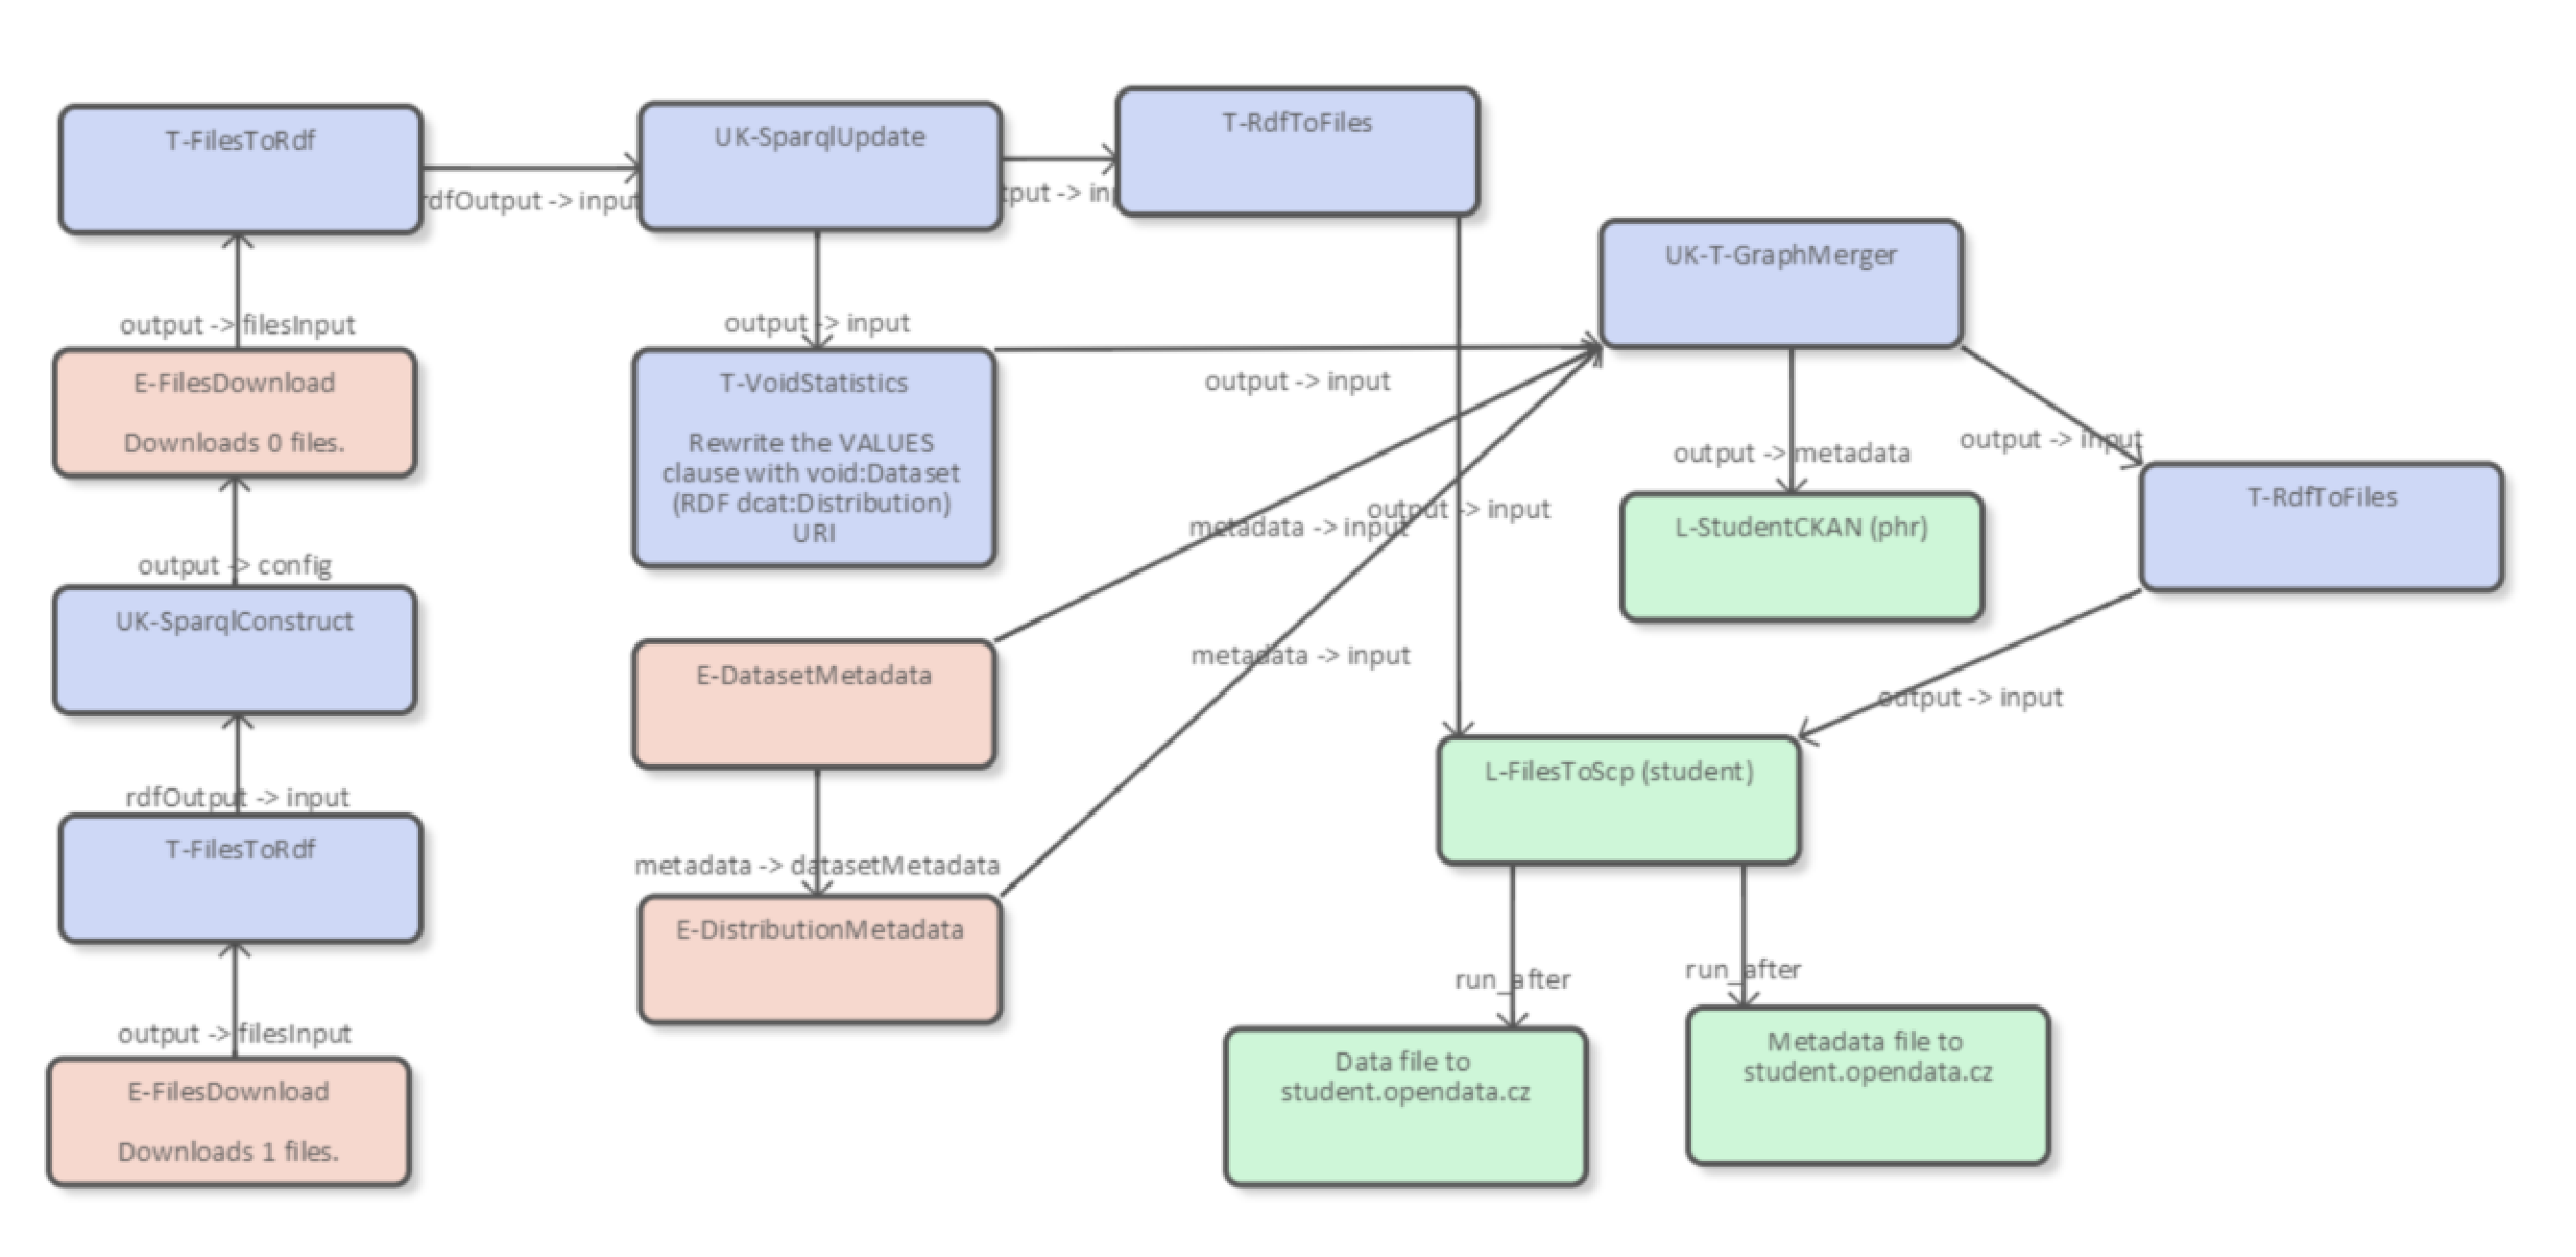
\includegraphics[width=\textwidth]{img/jednotneUloziste.eps}}
\caption{Pipeline nad jednotným úložištěm pro zpracování dat o smlouvách}
\label{obr:jednotneUloziste}
\end{figure}

\section{Webová aplikace}

\subsection{Volba technologií a implementační platformy}

Webová aplikace je implementována také v technologii ASP.Net se zvoleným architektonickým vzorem MVC. K práci s RDF daty využijeme také knihovnu dotnetRdf. Layout aplikace je tvořen formou responzivního Bootstrap\footnote{TODO} designu.

\subsection{Získávání dat}

V rámci aplikace využíváme přístup k datovým sadám z těchto SPARQL endpointů:

\begin{itemize}
\item Smlouvy - http://student.opendata.cz/sparql
\item Organizace, ARES, Orgány veřejné moci - http://linked.opendata.cz/sparql
\item RUIAN - http://ruian.linked.opendata.cz/sparql
\item DBpedia - http://dbpedia.org/sparql, nebo česká verze http://cs.dbpedia.org/sparql
\end{itemize}

Aplikace se skládá ze čtyř pohledů, Seznam mluv, Detail subjektu, Detail smlouvy a Veřejné zakázky subjektu. Konkrétní data se získají pomocí těchto SPARQL dotazů:

\subsubsection*{Seznam smluv}

\lstinputlisting[label=lst:getContracts, caption=Získej všechny smlouvy, language=XML]{code/getContracts.sparql}

\subsubsection*{Detail subjektu}

\lstinputlisting[label=lst:gePublisherName, caption=Získej vydavatele na základě jména, language=XML]{code/gePublisherName.sparql}

\lstinputlisting[label=lst:getContractByPublisherName, caption=Získej všechny smlouvy daného vydavatele úložiště, language=XML]{code/getContractByPublisherName.sparql}

\lstinputlisting[label=lst:getBusinessEntityOpeningHours, caption=Získej otevírací hodiny subjektu, language=XML]{code/getBusinessEntityOpeningHours.sparql}

\lstinputlisting[label=lst:getBusinessEntityRuianLink, caption=Získej adresní místo z RUIANu, language=XML]{code/getBusinessEntityRuianLink.sparql}

\lstinputlisting[label=lst:getBusinessEntityCoordinates, caption=Získej polohu subjektu, language=XML]{code/getBusinessEntityCoordinates.sparql}

\lstinputlisting[label=lst:getPublisherInfo, caption=Získej foto subjektu, language=XML]{code/getPublisherInfo.sparql}

\subsubsection*{Detail smlouvy}

\lstinputlisting[label=lst:getContract, caption=Získej smlouvu, language=XML]{code/getContract.sparql}

\lstinputlisting[label=lst:getPartiesByContract, caption=Získej smluvní strany na základě smlouvy, language=XML]{code/getPartiesByContract.sparql}

\lstinputlisting[label=lst:getAttachmentsContract.sparql, caption=Získej přílohy na základě smlouvy, language=XML]{code/getAttachmentsContract.sparql}

\lstinputlisting[label=lst:getAmendmentsByContract, caption=Získej dodatky na základě smlouvy, language=XML]{code/getAmendmentsByContract.sparql}

\lstinputlisting[label=lst:getMilestonesByContract, caption=Získej milníky na základě smlouvy, language=XML]{code/getMilestonesByContract.sparql}

\lstinputlisting[label=lst:getVersionsByContract, caption=Získej verzi smlouvy, language=XML]{code/getVersionsByContract.sparql}


\subsubsection*{Veřejné zakázky subjektu}

\lstinputlisting[label=lst:getBusinessEntityPublicContracts, caption=Získej veřejné zakázky na základě subjektu, language=XML]{code/getBusinessEntityPublicContracts.sparql}

